\chapter{Realisierung}\label{ch:realisierung}
In diesem Kapitel wird beschrieben, wie die Aufgabe dieser Arbeit gelöst wurde.
Dazu wird nach der im Kapitel \ref{ch:vorgehensweise} beschriebenen Reihenfolge, der Arbeitsschritte vorgegangen.
Es ist nochmal zu erwähnen, dass zunächst die Provisionierung einer CICS Instanz untersucht wird.
Danach wird in weiteren Schritten zuerst eine Db2 Datenbank und schließlich MQ Queues dem Bereitstellungsprozess hinzugefügt.
Die Funktionsfähigkeit der so generierten Laufzeitumgebung wird mittels eines Testablaufes sichergestellt.

\section{Testplex}
Vor Beginn der eigentlichen Untersuchung mussten zunächst alle benötigten Rechte beantragt werden.
Hierzu zählen unter anderem die Rechte für die Nutzung des Testplexes, die Nutzung von z/OSMF und z/OSPT und die Rechte für die Templateverwaltung innerhalb von z/OSMF.
Außerdem war es auf dem Testplex möglich, die Rechte für das Erstellen der CICS Dateien, das Recht, um ein CICS starten zu dürfen und die Rechte für die Administration von Db2 und MQ einer persönlichen UserID zu geben.
Dies stellt kein Problem dar, weil es sich bei dem Testplex um eine reine Systemtestumgebung handelt.
Außerdem benötigt das IBM Cloud and Management for z/OS lesenden Zugriff auf den Speicherpfad der Template Dateien.
Schließlich konnte mit dem ersten Versuch ein bei der Installation von z/OSMF mittgeliefertes minimales CICS Template zu provisionieren begonnen werden.

\subsection{IBM Standard CICS Template}
Trotz der Vorteile durch die Weboberfläche von z/OSMF wurde zunächst auf z/OSPT gesetzt.
Diese Entscheidung fiel auf Grund der höheren Flexibilität, durch Images.
Da es sich um ein mitgeliefertes Template handelt, sind alle benötigten Workflow Definitionsdateien und Template Dateien vorhanden.
Somit konnte der Konsolenbefehl `zospt build` auf dieses Template durchgeführt werden.
Dadurch sollte ein Image erzeugt werden.
Jedoch zeigte sich ein weiterer Nachteil des Kommandozeileninterfaces, es ist nicht möglich Templates eine Domain und einen Tenant zuzuweisen.
Dies hatte zur Folge das der Befehl `zospt build` fehlschlug.
Zusätzlich führte es dazu, dass für alle folgenden Aufgaben z/OSMF genutzt wird.

Das z/OSMF auf die Template- und Workflow-Dateien zugreifen kann, sind diese in einem Unix Dateisystem auf dem Großrechner gespeichert.
Das Template konnte dann ohne weitere Probleme in die Software Services aufgenommen werden.
Dabei wurden ihm eine Domain und ein Tenant zugewiesen.
Bevor das Template provisioniert werden kann, müssen Änderungen in der Eingabevariablen Datei vorgenommen werden.
Dazu mussten die Werte, der in Tabelle \ref{tab:cgsvars} genannten Variablen angepasst werden.
Die Kurzbeschreibungen und die Beschreibungen aller Variablen, die im Standard Template vorhanden sind, ist in \cite{IBM.2019} zu finden.
\begin{table}
\centering
\begin{tabularx}{\textwidth}{X|X}
Variablenname & Kurzbeschreibung \\
\hline
DFH\_REGION\_SEC & Legt fest, ob für das CICS Sicherheit im Allgemeinen aktiviert ist. \\
\hline
DFH\_REGION\_SECPRFX & Wenn DFH\_REGION\_SEC gesetzt ist, legt den Namen Perfix bei Authentificationanfragen für Ressourcen fest. \\
\hline
DFH\_REGION\_APPLID & Applikations ID der zu provisionierenden CICS Instance. \\
\hline
DFH\_LE\_HLQ & High-level qualifier\footnote{Erste Zeichen eines Dateinames, wird zum Filtern genutzt} für die Sprachumgebung\footnote{Grundeinstellungen der Programmiersprachen COBOL, PL1 und C. Mitgelieferte IBM Grundmodule} \\
\hline
DFH\_REGION\_HLQ & High-level qualifier für die CICS Dateien.\\
\hline
DFH\_REGION\_LOGSTREAM & Legt fest, wie die Log Dateien für das provisionierte CICS erstellt werden sollen. \\
\hline
DFH\_STC\_ID & User ID mit dem die CICS Instanz startet. \\
\hline
DFH\_REGION\_DFLTUSER & Default User ID für das CICS. \\
\hline
DFH\_REGION\_VTAMNODE & Name des VTAM Knotens, wenn das CICS hochfährt. \\
\hline
DFH\_REGION\_MEMLIMIT & Dem CICS maximal zur Verfügung stehender Speicherplatz. \\
\hline
DFH\_ZOS\_PROCLIB & Datei auf dem Großrechner, die den Job enthält, der für das Erzeugen der CICS Instanz zuständig ist. \\
\hline
DFH\_ZOS\_VSAM\_VOLUME & Speichersystem auf welchem die Dateien gespeichert werden sollen. Entscheidung kann auch an das System abgeben werden. \\
\hline
DFH\_CICS\_USSHOME & Homeverzeichnes des Unix System Services \\
\hline
DFH\_CICS\_HLQ & High-level qualifier von dem CICS Installationsort. \\
\end{tabularx}
\caption{Zu verändernde Variablen im minimalen CICS Template}
\label{tab:cgsvars}
\end{table}
Das diese Änderungen greifen, muss das Template aktualisiert werden.
Dies ist in der Oberfläche per Knopfdruck durchgeführt worden.

Als nächster Schritt wurde ein Testlauf und somit ein erster Versuch das Template zu provisionieren durchgeführt.
Hierbei trat beim ersten Step, der einen Job starten wollte, ein Fehler auf.
Nämlich um einen Rechte Verstoß bezüglich des Jobnames.
Bei der DATEV eG benötigt eine User ID die Rechte, um Jobs mit bestimmten Namen starten zu dürfen.
Da im Template von der IBM vorgeschlagene Jobnamen verwendet werden, kommt es zum Verstoß.
Um dieses Problem zu lösen, wurden die Jobnamen innerhalb des gesamten Templates an DATEV eG Standards angepasst.
Nachdem das Template aktualisiert wurde, wurde erneut versucht zu provisionieren.
Dabei stellte sich heraus, dass der Befehl, um ein CICS zu starten innerhalb der DATEV eG einen weiteren Parameter benötigt.
Dieser wurde hinzugefügt und danach funktionierte das Provisionieren und alle definierten Aktionen des minimalen IBM Standard CICS Templates.

\subsubsection{DATEV eG spezifischen CICS Template}\label{sssec:datevcics}
Nachdem das minimale IBM Standard CICS Template funktionsfähig war und erste Erfahrungen mit z/OSMF gesammelt wurden, wurde ein allgemeines mitgeliefertes Template untersucht.
Wie in der Tabelle \ref{vglTemps} dargestellt ist, ist dieses Template mit insgesamt 76 verwendeten Dateien sehr umfangreich.
Zu diesen Dateien zählen alle, die direkt mit dem Template in Verbindung stehen.
Das Template beinhaltet nicht nur die Möglichkeit verschiedene CICS Typen zu provisionieren, sondern auch, ob dies mit Skripten oder mit der REST-Api geschieht.
Dadurch verliert das Template an Übersichtlichkeit.
Zusätzlich kommt am Ende bei der Provisionierung keine CICS Instanz heraus, die einer DATEV eG spezifischen Instanz entspricht.
Auf Grund dessen wurden alle für ein DATEV eG spezifischen CICS nicht notwendigen Dateien entfernt.
Wie in der Tabelle \ref{vglTemps} zu sehen ist, hatte das unter anderem die Löschung von knapp der Hälfte der Dateien zur Folge.
Des Weiteren wurden auch viele nicht benötigte Variablen und Steps entfernt.
Dadurch schrumpft die provision.xml um circa ein Drittel.
Zusammenfassend lässt sich sagen, dass das Template an Übersichtlichkeit gewonnen hat.

Als nächstes wurde mit der Modifizierung der restlichen Dateien begonnen.
Als Ziel davon steht eine funktionsfähige DATEV eG spezifische CICS Instanz.
Zunächst wurden die Namen der CICS Dateien\footnote{Beschreibung in Absatz \ref{sssec:speziDat}} an die DATEV eG internen Namenskonventionen angepasst.

In Zusammenarbeit mit den CICS Administratorenteam wurde festgelegt, dass eine jede provisionierte CICS Instanz ihre eigene CSD Datei zur Verfügung gestellt bekommen soll.
Hierfür soll die bestehende von den Kollegen gepflegte Datei kopiert und mit bestimmten Namenkonventionen gespeichert werden.
Somit ist sichergestellt, dass durch die neu provisionierten Instanzen die Alten nicht beeinflusst werden.
Außerdem kann jeder Anwender so ohne Seiteneffekte seine CSD bearbeiten.
Ein weiterer Vorteil ist, dass bei der Deprovisionierung diese Kopie der Standard Datei ohne Nebenwirkungen gelöscht werden kann.
Dadurch dass die Datei, die von den Kollegen gepflegt wird als Grundlage verwendet wird, sind alle provisionierten Instanzen immer auf dem aktuellsten Stand.
Um dies Umzusetzen musste ein JCL Job geschrieben werden, der den Kopiervorgang abbildet.
Anschließend wurde dieser mittels eines neuen Steps in den Workflow eingebunden.
Außerdem mussten bestimmte Gruppen zu der CSD Liste der CICS Instanz hinzugefügt werden.
Die JCL ist in Abbildung \ref{code:addCSD} abgebildet.
Die Reihenfolge ist relevant, da es der Initialisierungsreihenfolge entspricht.

die JCL genau erkären..... bzw job im grundlagen teil erkären

Ein spezielles Augenmerk lag auf der Editierung der `createCICS.jcl`-Datei.
In dieser befindet sich die Definition des STC Jobs für das provisionierte CICS.
Im Standard IBM Template beinhaltet diese zunächst ein Makro für die Validierung von den SIT Parametern.
Noch bevor die Jobdefinition beginnt, werden alle aus der Datei für die Eingabevariablen benötigten Variablenwerte in temporäre Zwischenvariablen eingefügt.
Dadurch ist eine Änderung nur an einer Stelle notwendig, falls sich etwas an der Variablen ändert.
Danach folgt die Definition des Jobs, diese setzt sich aus folgenden Hauptbestandteilen zusammen:\\
\begin{itemize}
\item Einbindung der benötigten Bibliotheken
\item Einbindung der zuvor angelegten CICS spezifischen Dateien
\item Definition der SIT Parameter
\end{itemize}
In Abbildung \ref{HIER ABBILDUNG mit einlese von sitparams} ist zu sehen, dass es vor allem bei der Definition der SIT Parameter zu tief verschachtelten if-Bedingungen kommen kann.
Es handelt sich um den Code, der für das Einlesen der Variable `DFH\_REGION\_SITPARAMS` aus der Eingabedatei zuständig ist.
In dieser Variablen werden die SIT Parameter als Komma separierter String angegeben.
Für die Erzeugung eines DATEV eG spezifischen CICS, wurde das Makro für die Validierung von SIT Parametern beibehalten.
Alles danach wurde zunächst durch eine zur Verfügung gestellten DATEV eG Standard JCL, für die Erzeugung eines CICS, ersetzt.
Nach und nach ist die Logik, wie die aus Abbildung \ref{gleiche abbildung wie oben}, hinzugefügt worden.
Zusätzlich wurden die vorher statische DATEV eG Standard JCL durch Verwendung der Templatevariablen dynamisiert.

Zu der Definition der SIT Parameter ist zu sagen, dass hier nur die wirklich benötigten mit aufgenommen wurden.
Die anzunehmenden Werte wurden einzeln mit den CICS Administratorenteam besprochen und festgelegt.
Es ist zu beachten, dass es im IBM Standard Template zwei Möglichkeiten gibt, die Parameter zu setzen.
Für bestimmte SIT Parameter besteht eine Variable innerhalb des Templates.
Für alle anderen ist die Variable `DFH\_REGION\_SITPARAMS` vorgesehen.
In dieser Arbeit wurde hauptsächlich auf letztere Möglichkeit gesetzt.
Dadurch sind die SIT Parameter nur an einer Stelle im Template zu verwalten beziehungsweise die Verwaltung wird nicht auf zwei Arbeitsweisen verteilt.

Schließlich hat die Provisionierung eines DATEV eG spezifischen CICS Instanz funktioniert.
Dies wurde mit einem Anmeldevorgang an diese CICS sichergestellt.
Außerdem sind alle Standard DATEV eG Transaktionen funktionsfähig.
Es wurden alle Dateien wieder pflichtgerecht gelöscht.

\subsubsection{Bereitstellung Db2}\label{sssec:db2tpl}
In diesem Absatz wird die Provisionierung einer Db2 Datenbank beschrieben.
Da die Systemumgebung noch der Testplex ist, nur die Datenbank ohne Tabelle, ohne Daten.

Für die Erstellung einer Db2 Datenbank existiert innerhalb der DATEV eG eine REST-API.
Wie im Absatz \ref{sssec:workflow} beschrieben, ist es möglich innerhalb eines Workflow Steps einen REST-Request abzusenden.
Der Code ist in Abbildung \ref{code:db2prov} zu sehen.
So muss im Body des Requests unter anderem der Datenbankname und eine UserID übergeben werden.
Der Code für das Löschen der Datenbank sieht ähnlich aus, nur handelt es sich um einen DELETE-Request.
So wurden zwei neue Steps erzeugt und in den Workflow eingebunden.

Die API ist nur dazu fähig Datenbanken auf einem bestimmten Datenbanksystem zu erzeugen.
Um die Datenbank aus der CICS Instanz heraus nutzen zu können, muss dem CICS dieses Datenbanksystem mitgeteilt werden.
Hierfür ist, wie in Abbildung \ref{code:addCSD} bereits zu sehen ist, das Hinzufügen einer weiteren CSD Gruppe notwendig.
Des Weiteren müssen weitere Bibliotheken in der `createCICS.jcl` aufgenommen werden.
Um den Aufruf möglichst dynamisch zu gestalten wurden, zusätzlich neue Variablen im Template definiert.
Diese werden in der Eingabedatei des Templates gesetzt.

In Abilldung zeile SOUNSSO

\subsubsection{Bereitstellung MQ}\label{sssec:mqtplx}
In diesem Absatz wird die Provisionierung einer MQ Queue beschrieben.
Es ist auch möglich einen MQ Queuemanager zu provisionieren, der Fokus dieser Arbeit liegt aber auf der Bereitstellung von Queues.
Bei einem Queuemanager handelt es sich um ein Subsystem, deshalb wird vorerst von einer automatischen Bereitstellung abgesehen.
Auf dem Testplex wird des Weiteren die benötigte Funktion, dass eine CICS Transaktionen über eine Queue gestartet wird, nicht untersucht.
Außerdem wird zunächst nicht auf die Anforderungen der Anwendung eingegangen, sondern es wird geprüft wie es möglich ist eine einzelne Queue zu provisionieren.
Alles weitere wird erst in der Entwicklungssystemumgebung umgesetzt.
Dies ist im Absatz \ref{ssec:mqentw} beschrieben.

Die IBM stellt für die Verwaltung und das Nutzen von Queues Programme zur Verfügung.
Diese können mittels eines Jobs und bestimmten Parametern gestartet werden.
In Abbildung \ref{code:defq} ist die JCL des Jobs für das Erstellen einer Queue zu sehen.
Das auszuführende Programm ist `CSQUTIL` und als Parameter wird der Queuemanager übergeben.
Unter dem DD Namen `MQSCIN` ist der MQ Befehl für das Erzeugen einer Queue zu sehen.
Um zu Prüfen, ob die Queue auch funktionsfähig ist, wurde nach dem Erstellen auch mit Hilfe eines Jobs, eine Messages auf die Queue geschrieben und wieder abgeholt.
Der Job für das Löschen der Queues ist ähnlich aufgebaut.

Ähnlich wie in Absatz \ref{sssec:db2tpl} für die Datenbank beschrieben, muss der CSD Datei eine weitere Gruppe für den Queuemanager angegeben werden.
Dadurch hat die CICS Instanz auf alle Queues, die sich innerhalb dieses Managers befinden, Zugriff.
Des Weiteren ist die Aufnahme weiterer Bibliotheken in der `createCICS.jcl` notwendig.

\section{Entwicklungssystemumgebung}
Innerhalb der Entwicklungssystemumgebung sind die Sicherheits- und Rechtevorschriften schärfer als auf dem Testplex.
So wäre es zwar möglich alle für die administrativen Aufgaben notwendigen Rechte einer persönlichen UserID zu geben.
Dies würde bedeuten, dass alle Anwender dieses Templates diese Rechte auch benötigen.
Dies würde zu einem Chaos auf dem System führen, da sie auch außerhalb des Templates diese Rechte besitzen würden.
Somit wurde in Absprache mit den Administratorenteams für CICS und MQ festgelegt hierfür jeweils einen technischen User\footnote{User ID mit zunächst keinen Berechtigungen} zu beantragen.
Diesem werden nur die benötigten Rechte übergeben und ist somit sehr anwendungsspezifisch.
Um als Anwender das Template nutzen zu können, werden nur die Rechte benötigt Jobs mit diesen technischen Usern ausführen zu dürfen.
Für Db2 ist ein solcher User nicht notwendig, da das Datenbanksystem hinter der REST-API für alle zugänglich ist und jeder darauf Datenbanken erstellen darf.

Bei der Übertragung des Templates von der Testsystemumgebung auf die Entwicklungssystemumgebung waren Anpassungen in allen drei Bereichen des Templates notwendig.

\subsection{CICS Anpassung}
Zunächst wurden alle Steps modifiziert, so dass sie den CICS spezifischen technischen User verwenden.
Hierfür musste der `JOB` Baustein jeder JCL angepasst werden.
Dafür bietet zOSMF beim Zuweisen des `Tenants` eine Standard Jobkarte, die vor jeden Job des Templates eingefügt wird, hinterlegt werden.
Als nächstes musste ein Parameter bei der Erstellung der CICS spezifischen Dateien hinzugefügt werden.
Es handelt sich um den Massageclass Parameter mit dem Wert `NONE'.
Dadurch sind die Daten von der täglichen Datensicherung der Entwicklungssystemumgebung ausgenommen.
Da die Dateien bei der Deprovisionierung gelöscht werden, ist keine Sicherung notwendig.
Außerdem ändert sich die CSD Datei, die als Vorlage gilt, auf die Standard Entwicklungssystemumgebung CSD Datei.
Die Db2 und MQ Bibliotheken, die das CICS anzieht, besitzen einen anderen Namen.
So musste dies in der `createCICS.jcl` angepasst werden.
Zusätzlich musste ein SIT Parameter angepasst werden, so dass die Log Dateien funktionisfähig sind.
Außerdem kam noch ein Ordner neu hinzu.
Diese dient als später als Ablageort der kompilierten Programme.

\subsection{Db2 Anpassung}\label{ssec:db2entw}
Eine genauere technische Analyse, der Rechnungsschreibungsdatenbank, kam zum Ergebnis, dass es zwar möglich wäre diese Datenbank zu provisionieren, aber es den zeitlichen Rahmen dieser Arbeit übersteigen würde.
Der Grund hierfür ist die Komplexität, der benötigten Tabellen.
So wird auf drei Tabellen für die Ermittlung der Produktstammdaten lesend zugegriffen, auf neun weitere bei der Bestimmung der Preisabhänigkeiten.
Des Weiteren wird auf die Tabellen nicht direkt zugegriffen, sondern über Views.
Dabei werden nur bei drei Tabellen eins zu eins Views verwendet.
Bei allen anderen werden innerhalb der View noch weitere Tabellen, teilweise aus anderen Datenbanken, gejoint.
Insgesamt besteht das System aus 14 Tabellen, die auf vier Datenbanken aufgeteilt sind, und 12 Views für den Zugriff auf diese Tabellen.

Es wurde begonnen für die drei Produktstammdatentabellen, mit den Views und den dadurch zusätzlichen Datenbanken und Tabellen, die Definition in der Data Definition Language zu erstellen.
Es gibt keine Referenzen zwischen diesen Tabellen.
Es stellte sich heraus, dass diese Datei aus annähernd 600 Zeilen Code besteht.
Dieser ist im Anhang \ref{app:ddl} zu finden.
Dabei handelt es sich um ungetesteten Code.
Nachdem dieser Code getesten und die restlichen Tabellen, Views und Datenbanken ebenfalls aufgenommen wurden, müsste das ganze System noch mit den eigentlichen Daten befüllt werden.
Durch die Nutzung von Templates wäre dieser Aufwand einmalig zubewältigen, trotzdem überschreitet er diese Arbeit.

Für die weitere Arbeit werden, die in einem anderen Datenbanksystem bereits vorhanden, Datenbanken genutzt.
Hierfür musste der Wert, der dafür vorgesehenen Variablen in der Eingabedatei des Templates, geändert werden.
Außerdem wurden sowohl in der Provisionierungs- als auch in der Deprovisionierungsdatei die Datenbanksteps auskommentiert und somit kommen diese nicht mehr zum Einsatz.

\subsection{MQ Anpassung}\label{ssec:mqentw}
Da, wie im Absatz \ref{rechArch} beschrieben, sehr viele gleichartige Queues benötigt werden, wurde für die Erstellung dieser von den MQ Administratorenteam ein Rexx Skript angefertigt.
Dies geschah unabhänig dieser Arbeit zum Zeitpunkt der Einführung des Rechnungsschreibungsprozesses.
Dieses Skript steht dieser Arbeit zur Verfügung.
Es wurde auf die Bedürfnisse des Templates angepasst.

Hierfür wurden zunächst die Eingabeparameter durch vorher angelegte Templatevariablen ersetzt.
Diese steuern, wie viele Queues jeweils angelegt werden, auf welchen Queuemanager die Queues angelegt werden und den ersten Qualifier des Queuenamens.
Für den restlichen Queuenamen existiert auch eine Variable, in dieser werden die Namen als Komma separierte Liste angeben und ausgelesen.
An hand dieser Namen wird dann die maximale Queuetiefe und die maximale Länge einer einzelnen Nachricht festgelegt.
Im alten Skript wurden die Queues mit Hilfe einer Queue, die als Vorlage dient, angelegt.
Im Fall einer Provisionierung kann nicht davon ausgegangen werden, dass diese Vorlagen zur Verfügung stehen.
Deshalb wurden die benötigten Parameter händisch angegeben.
Um die so eben erstellten Queues zu testen, wurde eine Routine entwicklelt, die eine Nachricht auf die Queue schreibt und diese wieder abholt.
Anschließend wurde es in den Provisionierungsworkflow mit Hilfe eines neuen Steps aufgenommen.

Für die Deprovisionierung besteht noch kein Skript.
Als Grundlage dient das vorher angepasste Provisionierungsskript.
Hierfür musste der `Define`-Befehl für die Erstellung von Queues durch den `Delete`-Befehl ausgetauscht werden.
Die Logik für die Ermittlung der maximalen Queuetiefe und der maximalen Nachrichtenlänge wurde nicht mehr benötigt und konnte entfernt werden.

Diese beiden Skripte sind nur für den Datenaustausch zwischen der CICS Transaktion für die Preisermittlung und dem Batch Ablauf zuständig.
Wie in Absatz \ref{recharch} beschrieben, benötigt der Ablauf noch weitere Queues.
Da es sich hierbei um spezielle Queues handelt, wurde auf die im Absatz \ref{sssec:mqtplx} gezeigte Technik zurückgegriffen.
Bei der Antwort-Queue für die Ermittlung der Listenpreise handelt es sich um eine Queue ohne besondere Parameter.
Es werden noch zwei Trigger-Queues benötigt.
Die über Prozesse eine Transaktion im CICS starten.
Als letzter Baustein, dass das Triggering der Transaktion funktioniert, wird noch eine Initiation Queue benötigt.
Diese muss im CICS hinterlegt sein.

Jeder CICS Instanz kann nur eine Initiation Queue zugewiesen sein.
Dadurch benötigt jedes CICS eine eigene Initiation Queue.
Die Zuweisung geschieht in der MQ CSD Gruppe.
Somit müsste für jede provisionierte CICS Instanz im Voraus eine solche CSD Gruppe angelegt werden.
Daraus folgt, dass in diesem Schritt beschlossen wurde, die Verwaltung der MQ CSD Gruppe komplett dem Template zu übergeben.
Diese Entscheidung hatte eine Änderung des in Abbildung \ref{code:addCSD} gezeigten Codes zur Folge.
So wird, wie in Abbildung \ref{code:createGrp} abgebildet, zunächst eine Gruppe angelegt und erst anschließend dem CSD hinzugefügt.

Außerdem musste für jeden MQ bezogenen Job die Jobkarte angepasst werden, so wurden hier der technische User durch den technischen User, der für die administrativen MQ Aufgaben berechtigt ist, ausgetauscht.

\subsection{Testablauf}
Für die Prüfung der Funktionsfähigkeit der so generierten Laufzeitumgebung steht dieser Arbeit ein Testablauf zur Verfügung.
Dieser wurde von den Mitarbeitern der Rechnungsschreibung beigesteuert.
Dabei handelt es sich um einen Teilablauf des gesamten Rechnungsschreibungsprozesses.
In diesem Ablauf wird nur die Preisermittlung, die die Laufzeitumgebung benötigt, getestet.
Als Eingabe dienen vordefinierte Dateien und die Ergebnisse werden ebenfalls in Dateien geschrieben.
Der Ablauf liegt in Form von zwei Jobs vor.
Beide sind in der gleichen JCL Datei definiert, somit starten beide zeitgleich.
Dies ist notwendig, da der erste Job die Verarbeitung im CICS über die Queues startet und der Zweite lauscht auf die Ergebnisqueues.

Um den Ablauf auch auf der vorher provisionierten Laufzeitumgebung zu starten, musste lediglich der verwendete QueueManager angepasst werden.
Über die Queues und das verwendete Triggering wird die Transaktion im richtigen CICS gestartet.
Bei ersten Versuch den Ablauf zu starten kam es MQ-seitig zum Fehler.
Hier mussten noch zwei Queueparameter angepasst werden.
Danach ist der Testablauf ohne Fehler und mit der richtigen Ausgabe gelaufen.
Um die Ausgabe zu prüfen wurde der gleiche Testablauf mit den gleichen Eingabedateien auf der für Testzwecke üblichen Laufzeitumgebung durchgeführt.
Anschließend wurden die Ausgabedateien beider Läufe verglichen.

\section{Bereitstellungsprozess aktuelles Template}
Betrachtet wird der Fall eins, dass das Template dem Entwicklerteam im zOSMF zur Verfügung steht.
Es gibt noch keine Instanz dieses Templates.
Entwickler eins möchte einen neuen Programmstand testen und benötigt somit eine Instanz des Templates.
Der Mitarbeiter meldet sich an der zOSMF Oberfläche an und klickt auf den Menüleistenpunkt `Cloud Provisioing`.
Anschließend öftner er die `Software Services` und wählt dort das oben genannte Template aus.
Er kann es ohne Änderungen provisionieren und damit seine Programmabläufe testen.

Als nächstes wird der Fall zwei dargestellt bei dem bereits eine Instanz des Templates besteht.
Entwickler zwei möchte ebenfalls einen neuen Programmstand prüfen, unabhängig von den Änderungen aus Fall eins.
Somit benötigt er eine weitere Instanz des Templates.
Mit dem aktuellen Stand muss er wissen an welchem Speicherort das Template abgelegt ist.
Da er die Template- nicht die Workflowdateien kopieren muss.
Dann sind Änderungen an den Eingabevariablen des Templates notwendig.
Unter anderem ist eine andere CICS Application Id zu wählen.
Das die Queues und MQ Prozesse aus Fall eins nicht überschrieben werden, muss ebenfalls ein anderer Queue Manager gesetzt werden.
Anschließend muss mit den veränderten Dateien ein neues Template in zOSMF aufgenommen werden.
Schließlich kann Mitarbeiter zwei eine Instanz erzeugen.
Diese ist unabhängig von der Instanz aus Fall eins.

In Fall drei wird der Prozess, bei dem ein Administrator eine Änderung an einer Workflowdatei druchführt, betrachtet.
Zunächst muss der Speicherort der zu bearbeiteten Dateien bekannt sein.
Anschließend kann die Änderung mit einem Editor nach Wahl durchgeführt werden.
Jetzt sind noch zwei weitere Fälle zu betrachten.
Zunächst der Fall bei dem das Template noch nicht veröffentlicht wurde, dass heißt es steht noch keinem weiteren Team zur Verfügung.
Hier kann das Template in der zOSMF Oberfläche per Mausklick aktualisiert werden.
Bei dem nächsten Fall ist das Template bereits veröffentlicht.
Um die Funktionsfähigkeit der veralteten Instanzen weiterhin sicherzustellen, muss eine neue Version des Templates erzeugt werden.
Dies ist auch per Mausklick zu lösen.

\section{Fazit Realisierung}
Am Ende der Realisierung steht ein funktionsfähiges Template.
Dieses Template provisioniert ein CICS und die benötigten MQ Queues.
Wie in Absatz \ref{ssec:db2entw} beschrieben, wurde eine Db2 Datenbank wegen hoher Komplexität außen vorgelassen.
Es hat sich aber herausgestellt, dass dies theoretisch auch möglich wäre.
Zudem ist es möglich damit einen Testablauf der Rechnungsschreibung korrekt durchzuführen.

Jedoch gibt es auch Probleme.
Hier sind die nicht sprechenden Fehlermeldung, Abbildung \ref{fig:zosmffehler} als Beispiel, von zOSMF zu nennen.
\begin{figure}[h]
	\centering
	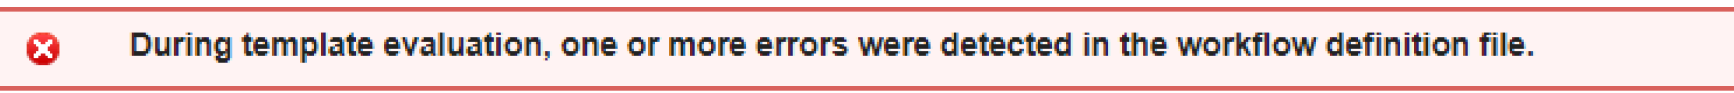
\includegraphics[width=\textwidth]{figures/zosmffehlermeldung.png}
	\caption{Beispiel einer Fehlermeldung von zOSMF}
	\label{fig:zosmffehler}
\end{figure}
So wird bei dem Hinzufügen und Aktualisieren eines Templates in zOSMF das Template und damit alle davon benötigten Dateien auf Syntaxfehler geprüft.
Die in Abbildung \ref{fig:zosmffehler} gezeigte Meldung tritt dann ein, wenn ein solcher Syntaxfehler vorhanden ist.
Es ist aber nicht zu erkennen, welcher Fehler genau vorliegt, noch nicht einmal in welcher Datei dieser auftritt.
Zudem auch keine genaue Anzahl an auftretenden Fehlern.
Dieser Umstand kombiniert mit 36 bestehenden Dateien gestaltet die Fehlersuche zeitaufwendig.
Im Gegensatz dazu wird im Fehlerfall beim Ausführen eines Steps immer der Fehlercode und der genaue Ort des Fehlers ausgegeben.
Zum Beispiel wird bei einem Step, in dem ein REST Aufruf gemacht wird, und ein Fehler auftritt, der Requestcode und die hinterlegte Fehlermeldung an der zOSMF Oberfläche angezeigt.

Ein weiteres Problem ist, die verwendete Programmiersprache, die für die dynamische Generierung von Skripten sorgt.
So ermöglicht diese die dynamische Wertzuweisung von zum Beispiel Rexxvariablen durch Templatevariablen.
Des Weiteren besteht eine Art von String Verarbeitung.
Zu beachten ist, dass wenn am Zeilenanfang ein `\#` steht, kann diese Programmiersprache verwendet werden.
In Abbildung \ref{Hier defineqrexx split} ist ein Beispiel zu sehen.
Dort werden die Queuenamen, die als kommaseparierte Liste in der Templatevariable `DFH\_MQ\_QUEUENAMES` angegeben sind, ausgelesen und in eigenen REXX Variablen gespeichert.
Zusehen ist zunächst eine `set` Anweisung mit der Variablen zugewiesen werden können.
Des Weiteren sind If-Bedingungen und eine foreach-Schleife zu sehen.
In Abbildung \ref{ergebnis split} wird das Ergebnis, welches zur Laufzeit ausgeführt wird, dargestellt.
Es ist zu erkennen, dass nur noch die für das REXX Skript notwendigen Codeabschnitte vorhanden sind.
Dadurch können sehr dynamische Templates erstellt werden.
Jedoch wurde weder eine Dokumentation zu dieser Sprache noch um welche Sprache es sich genau handelt gefunden.
Somit liegt dem Wissen über diese Sprache nur der Code aus Beispielen der IBM zu Grunde.

Ein weiterer Problempunkt ist das mit zOSMF und dem Template einhergehende Zugriffsrechtekonzept.
Die zOSMF Berechtigungsgruppen sind nicht an die DATEV eG internen Richtlinien angepasst.
Die Aufnahme in eine solche Gruppe, um zum Beispiel die zOSMF Oberfläche nutzen zu dürfen, geschieht auf Zuruf und händisches Hinzufügen einer User Id durch einen Mitarbeiter.
Außerdem ist der Einsatz einer für das ganze Template gültigen Standard Jobkarte, um technische User verwenden zu können, nicht optimal.
zOSMF bietet hier eigentlich eine Möglichkeit in der Stepdefinition einen `runAsUser` anzugeben.
Unter diesem User würde der Step dann ausgeführt werden, also die Stelle an der zum Beispiel für CICS Steps der technische User für administrative CICS Aufgaben angegeben werden müsste.
So wird das Gewehren der expliziten Rechte zum Starten eines Jobs mit der technischen User Id eingespart.
Dieses Gewehren ist wiederrum eine manuelle Arbeit, die mittels eines Formulares beantragt wird.
Jedoch um einen `runAsUser` in der Stepdefinition angeben zu können, muss in der dem Template zugewiesen `Domain` ein sogenannter `Cloud Security Admin` hinterlegt sein.
Dieser würde sicherstellen, dass nur die für ein Template zugelassenen User diesen Template auch provisionieren dürfen.
In dieser Arbeit wird die mitgelieferte `Default Domain` genutzt, in dieser ist kein `Cloud Security Admin` angegeben.
Da es sich um die Standard `Domain` handelt, darf diese nicht geändert werden.
Somit müsste eine eigene `Domain` angelegt werden um einen `Cloud Security Admin` hinterlegen zu können.
Dadurch dass sich zOSMF bei der DATEV eG noch in einem Teststadium befindet, wird von der Erstellung einer eigenen `Domain` abgesehen.
Dies ist der Grund für den nicht optimalen Einsatz von den oben genannten Jobkarten.
An diesen beiden Gründen ist zu erkennen, dass das Rechtekonzept noch nicht für einen firmenweiten Einsatz ausgelegt ist und noch überarbeitet und angepasst werden muss.
Dies ist nicht Bestandteil dieser Arbeit.

Je weiter das Projekt dem Abschluss näher kam desto mehr kristallisierte sich ein Hauptproblem heraus.
Dieses Template ist sehr auf die Rechnungsschreibung spezialisiert, dass heißt es ist funktionsfähig, aber kann nicht ohne zeitaufwendige Eingriffe in das Template, in die Workflowdefinitionsdateien und die eigentlichen REXX Skripte und Jobs, an eine andere Anwendung angepasst werden.
Bei der Betrachtung des Falles, wenn zwei Anwender jeweils eine eigene Instanz des gleichen Templates benötigen, muss dieses kopiert werden und neu in zOSMF aufgenommen werden.
Dies verlangt Wissen über die zOSMF Oberfläche und den Speicherort des Templates, um es schließlich auch zu ändern.
Da die Bereitstellung eines Queue Managers nicht im Template enthalten ist, müsste dafür ebenfalls ein Neuer angelegt werden.
Eine Herangehensweise an dieses Problem wird im Ausblick im Kapitel \ref{sec:techaus} dargestellt.